%(BEGIN_QUESTION)
% Copyright 2015, Tony R. Kuphaldt, released under the Creative Commons Attribution License (v 1.0)
% This means you may do almost anything with this work of mine, so long as you give me proper credit

\noindent
{\bf Laboratorieøvelse -- introduksjon}

\vskip 5pt

Oppgaven deres er å bygge, dokumentere og feilsøke et temperaturmålesystem bestående av en elektronisk temperaturtransmitter koblet til en elektronisk indikator, skriver eller indikerende regulator. Dere skal konfigurere transmitteren for både termoelementsensor {\it og} RTD-sensor, og deretter korrekt diagnostisere en feil plassert i et system teamet deres ikke har bygget selv. Omgivelsestemperatur i luft er anbefalt prosessvariabel, men andre variabler kan vurderes. Avvik fra standard temperaturmålelabb er kun tillatt etter godkjenning fra instruktør.

Tabellen under viser hvilke mål du og teamet ditt må fullføre innen planlagt tid for denne laboratorieøvelsen. Merk at noen mål er individuelle, mens andre gjelder hele teamet:

\underbar{Tabell for måloppnåelse:}

% No blank lines allowed between lines of an \halign structure!
% I use comments (%) instead, so that TeX doesn't choke.

$$\vbox{\offinterlineskip
\halign{\strut
\vrule \quad\hfil # \ \hfil & 
\vrule \quad\hfil # \ \hfil & 
\vrule \quad\hfil # \ \hfil & 
\vrule \quad\hfil # \ \hfil & 
\vrule \quad\hfil # \ \hfil & 
\vrule \quad\hfil # \ \hfil & 
\vrule \quad\hfil # \ \hfil \vrule \cr
\noalign{\hrule}
%
% First row
{\bf Prestasjonsmål} & {\bf Vurdering} & {\bf 1} & {\bf 2} & {\bf 3} & {\bf 4} & {\bf Team} \cr
%
\noalign{\hrule}
%
% Another row
Prototypeskisse ({\it før bygging av systemet!}) & mestring & -- & -- & -- & -- & \cr
%
\noalign{\hrule}
%
% Another row
Kretsdesign-utfordring & mestring & & & & & -- -- -- -- \cr
%
\noalign{\hrule}
%
% Another row
Endelig sløyfediagram og systeminspeksjon & mestring & & & & & -- -- -- -- \cr
%
\noalign{\hrule}
%
% Another row
RTD-signalsimulering ($\pm$ 1\% av span nøyaktighet) & mestring & & & & & -- -- -- -- \cr
%
\noalign{\hrule}
%
% Another row
T/C-signalsimulering ($\pm$ 1\% av span nøyaktighet) & mestring & & & & & -- -- -- -- \cr
%
\noalign{\hrule}
%
% Another row
Feilsøking & mestring & & & & & -- -- -- -- \cr
%
\noalign{\hrule}
%
% Another row
Labspørsmål: Instrumenttilkoblinger & proporsjonal &  &  &  &  & -- -- -- -- \cr
%
\noalign{\hrule}
%
% Another row
Labspørsmål: Idriftsetting & proporsjonal &  &  &  &  & -- -- -- -- \cr
%
\noalign{\hrule}
%
% Another row
Labspørsmål: Hoderegning & proporsjonal &  &  &  &  & -- -- -- -- \cr
%
\noalign{\hrule}
%
% Another row
Labspørsmål: Diagnostikk & proporsjonal &  &  &  &  & -- -- -- -- \cr
%
\noalign{\hrule}
%
% Another row
Avvikling og opprydding i lab & mestring & -- & -- & -- & -- &  \cr
%
\noalign{\hrule}
} % End of \halign 
}$$ % End of \vbox

Den eneste ``proporsjonale'' vurderingen i denne aktiviteten er labspørsmålene, som besvares individuelt av hver student. En liste over aktuelle labspørsmål finnes mot slutten av dette arbeidsarket. Spørsmålene skal både støtte labarbeidet og måle forståelsen deres, og instruktøren kan derfor stille spørsmålene fortløpende fra dag til dag i stedet for alt på én dag.

\vskip 10pt

{\bf Det er avgjørende at teamet planlegger hva som skal oppnås hver dag. Et kort teammøte (10 minutter) i starten av hver labøkt er en god måte å gjøre dette på: gå gjennom hva som er gjort, hva som gjenstår, og hvilke vurderinger dere må være klare for. Det er mye arbeid i å bygge, dokumentere og feilsøke fungerende instrumentsystemer!}

Etter hvert som dere jobber med systemet, vil dere uunngåelig møte problemer. Forsøk alltid å løse disse som team før dere ber instruktør om hjelp. Hvis dere fortsatt trenger hjelp, skriv teamfargen deres på labtavla med en kort beskrivelse av hva dere trenger hjelp til. Instruktøren følger opp teamene i den rekkefølgen de står på tavla.

$$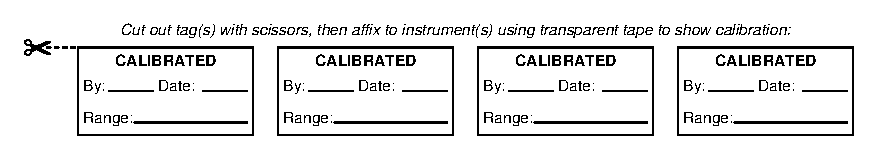
\includegraphics[width=15.5cm]{i00378x01.eps}$$



\vfil \eject

\noindent
{\bf Laboratorieøvelse -- valg av komponenter og planlegging av systemet}

\vskip 5pt

Et vanlig problem når studenter bygger fungerende systemer, enten på loddefritt brett eller som instrumentsløyfer i fullskala, er korrekt tilkobling og konfigurering av alle komponenter. En uheldig tendens er å starte koblingene uten en plan, altså å designe systemet underveis. Dette fører ofte til feilkoblinger og ikke-fungerende systemer, i noen tilfeller med ødelagte komponenter som følge av feil tilkobling.

En bedre metode er å planlegge først ved å designe systemet før bygging. Dette gjøres enkelt ved å lage en skisse som viser hvordan komponentene skal kobles, deretter analysere og forbedre skissen før noe kobles fysisk. Når dette gjøres i team, sikrer det at alle forstår hvordan systemet skal fungere og bygges. Prototypeskissen trenger ikke være svært kompleks, men må være detaljert nok til å vise hvilke terminaler/porter som kobles til hvilke. Skissen skal for eksempel tydeliggjøre at alle DC-komponenter får riktig polaritet. Dersom systemet inneholder mye rør/tubing, skal disse forbindelsene også vises.

\vskip 10pt

Første steg er å velge riktige feltinstrumenter fra instrumentlageret. I denne laben trenger dere en elektronisk temperaturtransmitter, enten ``smart'' eller analog. Rosemount modell 644/3044/3144/3244 er gode eksempler på smarte transmittere, mens Rosemount modell 444 er et godt eksempel på analog transmitter. Merk at analoge transmittere er laget for {\it enten} termoelement- eller RTD-inngang. Siden dere skal kalibrere {\it begge} typer i denne øvelsen, trengs to ulike analoge transmittere. Velger dere en ``smart'' transmitter, holder det normalt med én, fordi digitale temperaturtransmittere vanligvis kan konfigureres for både RTD og termoelement.

Neste steg er å finne relevant dokumentasjon for transmitteren. Nesten alle instrumenter i laben har elektronisk dokumentasjon hos produsent, så internett er beste kilde (og/eller Instrumentation Reference der mange manualer er lastet ned). Bruk dokumentasjonen til å finne korrekt tilkobling og kalibrering. Instruktøren vil kontrollere at dere har funnet og forstått manualen(e).

Etter valg av instrument og dokumentasjon bør dere gjøre en kvalitativ test før installasjon. For analog termoelementtransmitter kan dere kortslutte (jumpe) termoelementinngangen slik at transmitteren ``tror'' den måler romtemperatur. For analog RTD-transmitter kan dere koble 100 $\Omega$ motstand på RTD-terminalene slik at transmitteren ``tror'' den måler frysepunktet til vann. For digital (``smart'') transmitter: konfigurer først for 2-leder RTD eller termoelement med HART-kommunikator, og gjør deretter tilsvarende tester. Hvis transmitteren ikke responderer riktig, merk den med etikett som forklarer hva den gjør (eller ikke gjør).

\vskip 10pt

Prototypeskissen er så viktig at instruktøren krever den før bygging starter. {\it Team som bygger uten godkjent plan, blir stoppet og får ikke fortsette før plan er utarbeidet og godkjent!} Hvert teammedlem bør ha tilgang til planen (helst egen kopi) gjennom hele byggeprosessen. Prototypeskisser er en faglig vane dere bør ta med videre i yrket.

\vskip 10pt

{\bf Planlegging av et fungerende system bør ikke ta mer enn én time når teamet jobber effektivt, og kan spare dere for mange timer frustrasjon (og mulig ødeleggelse av komponenter)!}





\vfil \eject

\noindent
{\bf Laboratorieøvelse -- kretsdesign-utfordring}

\vskip 5pt

Koble en sløyfedrevet temperaturtransmitter (4--20 mA-utgang) til DC-spenningskilde og måleinstrument slik at instrumentet viser økende signal når temperaturføleren varmes opp. Alle elektriske koblinger skal utføres med rekkeklemmer (ingen tvinnede ledninger, skjøtehylser, wire nuts, fjærklemmer eller ``krokodilleklemmer'').

Øvelsen tester evnen til å koble strøm korrekt til sløyfedrevet transmitter, koble flere batterier for nødvendig forsyningsspenning, identifisere ulike termoelement- og RTD-typer, koble termoelement/RTD korrekt til transmitter, kondisjonere signalet (ved behov) slik at instrumentet kan lese det riktig, koble analogt måleinstrument korrekt i kretsen, og bruke rekkeklemmer for ryddig tilkobling.

$$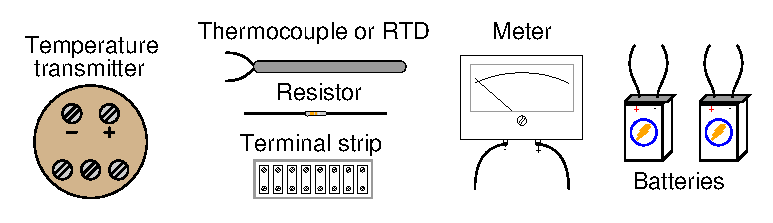
\includegraphics[width=15.5cm]{i00378x04.eps}$$

\vskip 10pt

Følgende komponenter/materialer er tilgjengelige: ulike 2-leder 4--20 mA temperatur-{\bf transmittere} kalibrert til områder som inkluderer romtemperatur; ulike {\bf termoelementer} og {\bf RTD-er}; {\bf rekkeklemmer}; lengder med {\bf koblingsledning}; 250 $\Omega$ (eller tilsvarende) {\bf motstander}; analoge {\bf målere}; {\bf batteriklemmer} (holdere).

\vskip 10pt

Dere må selv stille med skrutrekkere og multimeter for bygging og test ved pulten. Instruktøren leverer batteri(er) når dere er klare for funksjonstest. Inntil da skal kretsen være spenningsløs.

\vskip 10pt

\noindent
{\bf Måleralternativer} (instruktør velger): \hskip 20pt \underbar{\hskip 20pt} Voltmeter (1--5 VDC) \hskip 20pt \underbar{\hskip 20pt} Amperemeter (4--20 mA)

\vskip 10pt

\noindent
{\bf Sensortype} (instruktør velger): \hskip 20pt \underbar{\hskip 20pt} Termoelement \hskip 20pt \underbar{\hskip 20pt} RTD

\vfil

Studereferanse: kapitlet ``Analog Electronic Instrumentation'' i {\it Lessons In Industrial Instrumentation}, særlig om sløyfedrevne transmittere og feilsøking av strømsløyfer. Se også kapitlet ``Continuous Temperature Measurement'', spesielt delene om termoelementer og RTD-er.



\vfil \eject

\noindent
{\bf Laboratorieøvelse -- bygging av systemet}

\vskip 5pt

Instrumenteringslabben er lagt opp for å bygge fungerende instrumentsløyfer, med mange koblingsbokser, ferdigtrukne signalkabler og ``racks'' med 2-tommers vertikale rør for instrumentmontasje. De eneste ledningene dere normalt trenger å legge, er fra feltinstrument til nærmeste koblingsboks, samt korte ``jumper''-kabler mellom ferdiginstallerte kabler i mellomliggende koblingsbokser.

Når prototypeskissen er godkjent av instruktøren, kan byggingen starte. Transmittere monteres på 2-tommers rør med spesialbraketter og U-bolter. Disse finnes sammen med transmitterne i instrumentlageret.

Velg en konkret sløyferegulator som skal fungere som indikator for målt temperatur. Instruktøren kan tildele regulator for å sikre at dere lærer mer enn én regulatorvariant i løpet av perioden.

Til slutt må temperaturmålesystemet få et sløyfenummer, slik at alle instrumenter kan merkes korrekt. Nummeret må være unikt slik at ingen andre team bruker samme merkingen. En enkel metode er å bruke motstandsfargekoden for teamfargen i sløyfenummeret. Er dere ``rødt'' team, kan sløyfenummeret for eksempel være ``2''.

\vskip 10pt

{\bf Vanlige feil:}

\begin{itemize}
\item{} Ikke bruke produsentens dokumentasjon for feltinstrumenter (f.eks. kobling og kalibrering).
\item{} Montere feltinstrumenter i uhensiktsmessige posisjoner, slik at terminaler/deksler blir vanskelige å nå.
\item{} Ikke dra i hver eneste leder ved terminering for å kontrollere mekanisk god forbindelse.
\item{} Studenter jobber isolert på hver sin del uten å dele hva de har gjort. Hele teamet må lære alle deler av systemet.
\end{itemize}

{\bf Bygging av fungerende system bør ikke ta mer enn én full labøkt (3 timer) dersom komponenter er tilgjengelige og teamet jobber effektivt!}



\vfil \eject

\noindent
{\bf Laboratorieøvelse -- dokumentasjon av systemet}

\vskip 5pt

Hver student skal lage sitt eget {\it sløyfediagram} for teamets system etter ISA-konvensjoner. Eksempel på sløyfediagram vises i neste oppgave i dette arbeidsarket. Diagrammene må være {\it komplette} og {\it detaljerte}, med alle lederkoblinger, kabler, rekkeklemmer, områdepunkter osv. Målet er et så entydig diagram at enhver person kan følge det og koble riktig, også uten dyp instrumenteringsforståelse. I industrien bygges ofte sløyfer av innleid personell med begrenset prosessforståelse; diagrammet må derfor være presist nok til korrekt utførelse også da.

Alle instrumenter og signalkabler i sløyfen skal merkes med ISA-standard tagnummer. En enkel metode er kort bit maskeringsteip rundt hver kabel (og på hvert instrument), med permanent tusj. Det finnes ingen universell industristandard for kabelmerking, men en god praksis er å merke hver toleder med tagnummeret til feltinstrumentet den går til. Alle tolederkabler i en temperaturtransmitterkrets kan for eksempel merkes ``TT-$x$'' (der ``$x$'' er sløyfenummer). Hele sløyfen defineres av prosessvariabelen den måler: er PV {\it temperatur}, blir transmitter en {\it T}T, ventil en {\it T}V, regulator en {\it T}C, osv.

Når hele teamet er ferdig med individuelle sløyfediagrammer, tilkalles instruktør for sløyfeinspeksjon. Studentene går da systemet i tur og orden, mens de andre kontrollerer diagrammer for feil og mangler. Instruktøren kontrollerer samtidig installasjonskvalitet: frynsete ledere, feil crimping, dårlig kabelføring, manglende merking, manglende wire-duct-lokk osv. Teamet må rette alle avvik for å få godkjent systemet.

Etter godkjent inspeksjon skal hvert teammedlem legge sløyfediagrammet i diagramholderen midt i laben bak hovedpanelet. Når dere senere skal feilsøke et annet teams system, er dette stedet dere henter sløyfediagrammet.

\vskip 10pt

{\bf Vanlige feil:}

\begin{itemize}
\item{} Glemme merking av alle signalledere (se eksempel på sløyfediagram).
\item{} Glemme merking av alle feltinstrumenter med egne tag-navn (f.eks. TT-83).
\item{} Glemme å notere alle lederfarger.
\item{} Glemme navn på sløyfediagrammet.
\item{} Basere eget diagram på en lagkamerats i stedet for å kontrollere systemet selv.
\item{} Ikke plassere instrumentsymboler i riktig orientering (feltinstrumenter til venstre, kontrollromsinstrumenter til høyre).
\end{itemize}

\vskip 10pt

{\bf Utarbeidelse og inspeksjon av korrekte sløyfediagrammer bør ikke ta mer enn én full labøkt (3 timer) hvis teamet jobber effektivt!}




\vfil \eject

\noindent
{\bf Laboratorieøvelse -- instrumentkalibrering}

\vskip 5pt

Hvert team må kalibrere transmitteren slik at den tolker temperatur korrekt og gir korrekt strøm ut, og samtidig skalere indikator (eller indikerende regulator) i riktige ingeniørenheter (f.eks. transmitter satt 0--200 $^{o}$F skal faktisk vises som 0--200 $^{o}$F i kontrollrom). Teamet bør velge et temperaturintervall som inkluderer romtemperatur, men som {\it ikke} er 0--100, slik at dere trener på å sette områdepunkter til andre verdier enn standard 0--100\%. Team som bruker ``smart'' transmitter må ``trimme'' både inngang og utgang og deretter sette område (LRV/URV). Team med analog transmitter må påføre LRV/URV-elektriske signaler og justere ``zero''- og ``span''-potensiometre.

Som alltid ved kalibrering må instrumentets respons sammenlignes med én eller flere {\it standarder}. Her bruker vi enten millivolt (termoelement) eller motstand (RTD) inn på temperaturtransmitter med termoelement/RTD-simulator, mens multimeter måler transmitterutgang i DC mA:

$$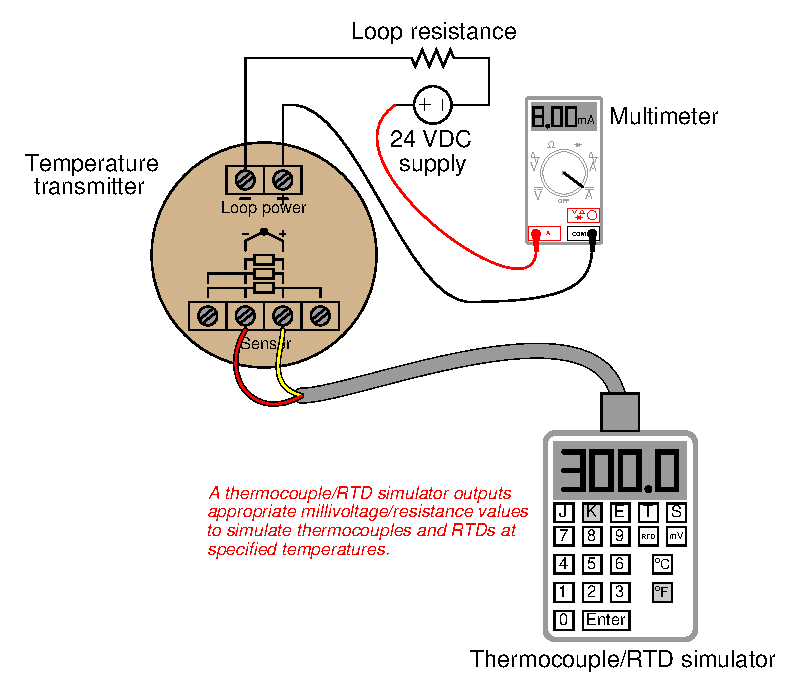
\includegraphics[width=15.5cm]{i00378x02.eps}$$

Kalibrering kan utføres på kalibreringsbenk/arbeidsbord eller i felt. Se simulatorens dokumentasjon for korrekt tilkobling til aktuell transmitter. Dette er særlig nyttig ved simulering av 3- eller 4-leder RTD.

\filbreak

Dokumenter nøyaktigheten til transmitterens sensortrim før og etter justering i tabellen under, ved fem punkter i måleområdet. ``Påført'' temperatur er temperaturen dere simulerer med termoelement/RTD-simulator, og ``Indikert'' temperatur er det HART-kommunikatoren viser som prosessvariabel (eller tilsvarende temperatur utledet fra 4--20 mA-utgangssignal):

% No blank lines allowed between lines of an \halign structure!
% I use comments (%) instead, so that TeX doesn't choke.

$$\vbox{\offinterlineskip
\halign{\strut
\vrule \quad\hfil # \ \hfil & 
\vrule \quad\hfil # \ \hfil & 
\vrule \quad\hfil # \ \hfil \vrule \cr
\noalign{\hrule}
%
% First row
Påført temperatur & Indikert temperatur (As-Found) & Indikert temperatur (As-left) \cr
%
\noalign{\hrule}
%
% Another row
 &  & \cr
%
\noalign{\hrule}
%
% Another row
 &  & \cr
%
\noalign{\hrule}
%
% Another row
 &  & \cr
%
\noalign{\hrule}
%
% Another row
 &  & \cr
%
\noalign{\hrule}
%
% Another row
 &  & \cr
%
\noalign{\hrule}
} % End of \halign 
}$$ % End of \vbox

Når kalibreringen er ferdig, sett kalibreringsmerke på transmitteren med område og kalibreringsdato. Førstesiden i denne labøvelsen har klippbare kalibreringslapper som kan teipes på transmitteren.

\vskip 10pt

Etter at teamet har kalibrert og installert transmitteren, skal hver student individuelt demonstrere forståelse av signalene fra termoelement og RTD ved manuelt å simulere passende signal på transmitterinngangen, slik at tilfeldig temperatur verdi oppgitt av instruktør vises korrekt. Formålet er å sikre at hver student forstår hvordan termoelementer og RTD-er faktisk virker, samt bruken av tabeller for disse sensorene.

For eksempel: Hvis teamet kalibrerer/installere type J-termoelementtransmitter med område 0--150 $^{o}$F, velger instruktøren ulike temperaturer innen området (f.eks. 102, 93, 77, 128 $^{o}$F) som hver student skal simulere med enkel elektrisk utrustning (ingen termoelement/RTD-simulator tillatt i denne delen). ``T/C signal simulation'' bestås når studenten klarer å simulere spesifisert temperatur med kun multimeter og lavspenningskilde (f.eks. DC-forsyning med spenningsdeler). ``RTD signal simulation'' bestås når studenten simulerer spesifisert temperatur med kun multimeter og lavohmig variabel motstand (f.eks. potensiometer eller dekademotstand). Instruktøren kontrollerer at oppgitt temperatur vises innen $\pm$ 1\% av transmitterens span.

\filbreak

Illustrasjonene under viser prinsipp for termoelement- (``T/C'') og RTD-signalsimulering. Motstandsverdiene er kun eksempler, og må eventuelt tilpasses applikasjonen. {\it Sett av tid til at alle i teamet virkelig forstår hvordan og hvorfor disse potensiometernettverkene fungerer som termoelement-/RTD-simulatorer}:

$$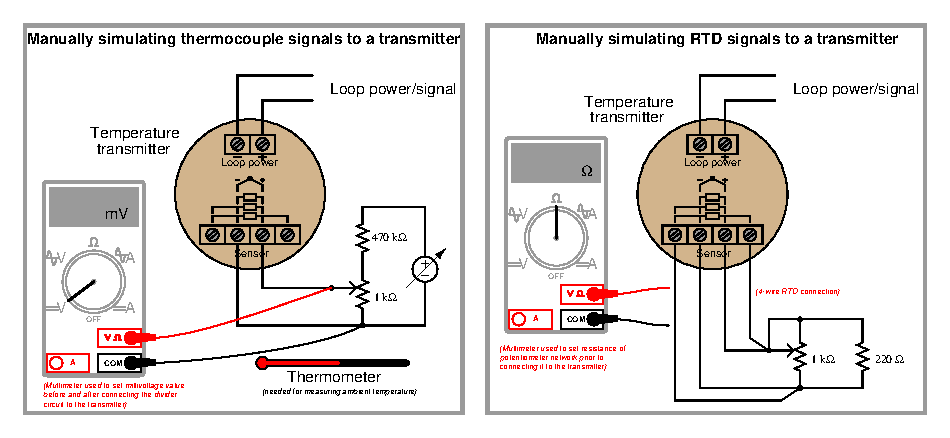
\includegraphics[width=15.5cm]{i00378x03.eps}$$

Det anbefales å bruke rekkeklemmer i stedet for loddefritt breadboard ved bygging av potensiometernettverk, på grunn av ustabil kontaktmotstand i breadboard. Bruk ``relative''-funksjonen på DMM motstandsområde for å nullstille motstanden i måleledningene ved innstilling av RTD-simuleringsnettverk. Hvis DMM har ``high resolution'' for millivolt, bruk den ved innstilling av termoelement-simuleringssignal.

Studenter opplever ofte termoelementsimulering som mer krevende enn RTD-simulering: RTD representerer en bestemt motstand ved hver temperatur, mens termoelementsignal avhenger av både prosesstemperatur {\it og} omgivelsestemperaturen ved transmitterterminalene. For mer informasjon, se ``Thermocouples'' i kapitlet ``Continuous Temperature Measurement'' i {\it Lessons In Industrial Instrumentation}.

\vskip 10pt

{\bf Vanlige feil:}

\begin{itemize}
\item{} Påføre for høy spenning på inngangen til termoelement- eller RTD-transmitter. Husk at termoelementer bare gir små spenninger i lavt millivoltområde. Studenter har {\bf ødelagt} transmittere ved å legge så lite som 1.5 volt på inngangen, i tro om at det var trygt. For å unngå dette: sett millivoltsignalet i simuleringskretsen {\it før} tilkobling til transmitterinngangen.
\item{} Ikke måle omgivelsestemperatur nøyaktig ved manuell termoelementsimulering (for korrekt referanseskjøt-millivolt).
\item{} Feiltolke rader/kolonner i termoelement-/RTD-tabeller ved oppslag av millivolt- eller motstandsverdier.
\item{} Velge kalibreringsområde (``trim'') som er betydelig mindre enn sluttområdet i drift. Som hovedregel bør sensortrim dekke bredest mulig område med tilgjengelig kalibreringsutstyr.
\item{} Glemme å sette kalibreringsmerke på transmitter etter kalibrering.
\end{itemize}

\vskip 10pt

{\bf Kalibrering av teamets transmitter bør ikke ta mer enn én full labøkt (3 timer) dersom teamet jobber effektivt!}



\vfil \eject

\noindent
{\bf Laboratorieøvelse -- feilsøking}

\vskip 5pt

Den mest krevende delen av øvelsen er {\it feilsøking}, der du skal vise evne til logisk isolering av feil i systemet. All feilsøking vurderes individuelt (ingen teampoeng), og skal utføres {\it på et system du ikke har vært med å bygge}, slik at du må bruke sløyfediagram aktivt i stedet for minne fra bygging.

Hver student får 5 minutter til å identifisere både generell plassering og type feil, og samtidig begrunne alle diagnostiske steg logisk. All feilsøking gjennomføres under direkte oppsyn av instruktør for å sikre selvstendig og effektiv gjennomføring.

Hvis studenten ikke identifiserer både feilplassering og feiltype innen tidsfristen, og/eller ikke viser rasjonell diagnostisk metode, blir forsøket underkjent. Studenten må da prøve på nytt med en annen feil. Flere nye forsøk er tillatt uten trekk i karakter.

Kun standard multimeter er tillatt testutstyr i tidsvinduet. Kretsbrudd for diagnostikk er ikke tillatt uten instruktørens tillatelse, og da bare etter korrekt forklaring av hvilke problemer dette kan skape i et virkelig anlegg.

Instruktøren gjennomgår hvert forsøk i etterkant og peker på sterke/svake sider for læring. Feilsøking er en ferdighet som bygges gjennom øvelse og feil, så ikke bli motløs hvis flere forsøk trengs. En viktig livslære i aktiviteten er å håndtere nederlag, fordi dette {\it vil} forekomme i arbeidslivet. Det er ingen skam å ikke lykkes på første forsøk når du gjør et seriøst arbeid. Det som ikke er akseptabelt, er snarveier eller å gi opp.

\vskip 10pt

{\bf Vanlige feil:}

\begin{itemize}
\item{} Unnlate å ta målinger med multimeter.
\item{} Unnlate å kontrollere andre målinger i systemet (f.eks. temperaturmåleravlesning).
\item{} Ikke utnytte raske tester som ``input short test'' (jumpe inngang på termoelement-/RTD-transmitter for å sjekke respons) ved mistanke om transmitterfeil.
\item{} Feiltolke sløyfediagram (f.eks. tro at målingen tas på feil sted).
\item{} Feil bruk av multimeter (f.eks. AC i stedet for DC, feil område, feil plassering av måleledninger), særlig når student låner ukjent måler.
\end{itemize}

\vskip 10pt

{\bf Husk at hensikten med feilsøkingsøvelsen er å utvikle og vurdere evnen til intelligent diagnose av komplekse systemer. Å finne feilen ved flaks eller ren prøve-og-feile-kontroll er ikke en godkjent ferdighetsdemonstrasjon. Det som teller, er dokumentert evne til logisk analyse og isolering av problemet, med korrekt forklaring av alle steg!}

\vskip 10pt

{\bf Feilsøking krever mye labtid, ofte minst to 3-timers økter for at en full klasse skal komme i mål. Teamet må budsjettere tid til dette i planen, og dere bør benytte muligheten til å observere andre under feilsøking for å lære metoden bedre.}



\vfil \eject

\noindent
{\bf Labspørsmål}

\vskip 5pt

\begin{itemize}
\item{} {\bf Instrumenttilkoblinger}
\item{} Bestem korrekte ledningsforbindelser mellom instrumenter for å lage en fungerende 4--20 mA sløyfe, basert på diagrammer med merkede terminaler
\item{} Identifiser korrekt alle elektriske kilder/laster, spenningspolaritet og strømretning i 4--20 mA sløyfekrets, basert på diagrammer med merkede terminaler
\end{itemize}

\filbreak

\begin{itemize}
\item{} {\bf Idriftsetting og dokumentasjon}
\item{} Identifiser fargekoder og metalltyper for type J-termoelement
\item{} Identifiser fargekoder og metalltyper for type K-termoelement
\item{} Identifiser fargekoder og metalltyper for type T-termoelement
\item{} Identifiser fargekoder og metalltyper for type S-termoelement
\item{} Identifiser fargekoder og metalltyper for type E-termoelement
\item{} Ranger type J, K, T, S og E etter maksimale temperaturer
\item{} Forklar hva kuldeskjøt- (eller referanseskjøt-) kompensasjon er, og hvorfor det er nødvendig
\item{} Forklar hvordan termoelementkvalitetsledning skilles fra forlengelsesledning
\end{itemize}

\filbreak

\begin{itemize}
\item{} {\bf Hoderegning} (kalkulator ikke tillatt!)
\item{} Beregn riktig sløyfestrøm (mA) gitt transmitterområde og påført temperatur
\item{} Beregn påført temperatur gitt transmitterområde og målt sløyfestrøm
\item{} Beregn prosent av span-feil for transmitter gitt område og As-Found-kalibreringstabell
\item{} Beregn tillatt temperaturfeil for transmitter gitt tillatt prosent av span-feil og område
\item{} Konverter mellom temperaturenheter uten å bruke oppslagsverk for konverteringsfaktorer (hovedfaktorer må kunne huskes)
\end{itemize}

\filbreak

\begin{itemize}
\item{} {\bf Diagnostikk}
\item{} Forklar hva som skjer (og hvorfor) hvis termoelementkrets får {\it kortslutning} et bestemt sted i ledningsnettet
\item{} Forklar hva som skjer (og hvorfor) hvis RTD-krets får {\it brudd} eller {\it kortslutning} et bestemt sted i sensorledningen
\item{} Vurder om en gitt diagnostisk test gir nyttig informasjon ut fra symptomsett i et feilet system
\item{} Identifiser minst to plausible feil gitt diagnostisk testresultat og symptomsett i et feilet system
\item{} Foreslå en diagnostisk test og forklar betydningen av to ulike mulige testresultater
\end{itemize}


\vfil \eject

\noindent
{\bf Laboratorieøvelse -- avvikling og opprydding}

\vskip 5pt

Siste steg i øvelsen er å avvikle hele teamets system og tilbakeføre utvalgte komponenter til riktig lagringsplass for å klargjøre laben for neste øvelse. Fjern systemdokumentasjon (f.eks. sløyfediagram) fra felles oppbevaringsområde, og kast eller behold for egne notater. Fjern også instrumentmerking (f.eks. FT-101) fra instrumenter og kabler. Utfør generell opprydding i labområdet: kast avfall, legg verktøy på riktig plass, rydd ledningsrester fra gulv og koblingsbokser osv.

\vskip 10pt

\indent
{\bf La følgende komponenter stå montert på rackene:}

\begin{itemize}
\item{} Store reguleringsventiler og posisjonere
\item{} I/P-omformere
\item{} Store elektriske motorer
\item{} Store frekvensomformere (VFD)
\item{} Kabler i rør mellom koblingsbokser
\item{} Rør- og tubefittings (ikke skru opp gjengede rørkoblinger)
\item{} Forsyningsregulatorer for instrumentluft
\end{itemize}

\vskip 10pt

\indent
{\bf Returner følgende komponenter til riktig lagringsplass:}

\begin{itemize}
\item{} Følerelementer (f.eks. termoelementer, pH-prober osv.)
\item{} Prosess-transmittere
\item{} ``Jumper''-kabler mellom rekkeklemmer i samme koblingsboks
\item{} Plasttubing og tube-fittings (koble fra kompresjonsfittings)
\item{} Strømkabler og skjøteledninger
\item{} Justerbare lufttrykksregulatorer (loading station)
\end{itemize}

\vskip 10pt

Til slutt skal alle komponenter i styringssystemet tilbakeføres til original standardkonfigurasjon (fabrikkstandard). Dette inkluderer PID-innstillinger, funksjonsblokkprogram, inngangsområder osv.




\underbar{file i00378}
%(END_QUESTION)





%(BEGIN_ANSWER)


%(END_ANSWER)





%(BEGIN_NOTES)

\noindent
{\bf Sløyfediagram / inspeksjon:}

Jeg anbefaler sterkt å krysse av studentenes sløyfediagrammer mens sløyfen inspiseres (sikre ledningsforbindelser, korrekt tubing, god føring i rør osv.). La alle teammedlemmer ta deg med på en ``omvisning'' i ferdig sløyfe, der hver student forklarer en valgt del med eget sløyfediagram som støtte. Mens én forklarer, kan du kontrollere de andres diagrammer for nøyaktighet. Dette sparer tid ved å kombinere inspeksjon og diagramkontroll, og sikrer at studentene faktisk kan knytte diagrammet til den bygde sløyfen og formidle forståelsen.

\vskip 10pt

\goodbreak

\noindent
{\bf Forslag til feilsøkingsfeil:}

\begin{itemize}
\item{} Avisoler leder ved terminal, men klem fast isolert del i stedet for blank leder (lederbrudd)
\item{} Kutt signalkabel et sted i rørføring (lederbrudd)
\item{} Trykk en tegnestift gjennom kabel i rørføring (kortslutning)
\item{} Koble instrumentkabelledere omvendt (byggefeil)
\item{} Koble termoelementkabelledere omvendt (byggefeil)
\item{} Kortslutt termoelementkabel i frakoblingsplugg med tynn kobbertråd
\item{} Sett transmitter med for høy demping (treg respons)
\item{} Sett indikator/regulator med for høy demping (treg respons)
\item{} Feilkalibrer transmitter og/eller indikator/regulator (unøyaktighet)
\item{} Reversér virkemåte på regulator/posisjonerer/transmitter (feil respons)
\item{} Koble 2.2 k motstand parallelt med 4--20 mA-transmitter for å simulere delvis kortslutning i kabling (unøyaktighet)
\item{} Bytt 250 ohm motstand med en som ser lik ut, men har feil verdi (unøyaktighet)
\item{} Koble fra kabel(r) inni transmitter eller regulator (instrumentfeil)
\item{} Del ut feil sløyfediagram til studentene (dokumentasjonsfeil)
\item{} Lukk ventil og la sikkerhetstag henge på (operatør-/teknikerfeil)
\end{itemize}






\vfil \eject

\noindent
{\bf Labspørsmål}

\vskip 20pt
\begin{itemize}
\item{} Identifiser fargekoder og metalltyper for type T-termoelement.

\vskip 20pt

\item{} Forklar {\it i detalj} hvordan vann kan brukes som temperaturkalibreringsstandard.

\vskip 20pt

\item{} Beregn strømutgangen fra en temperaturtransmitter med område 0 til 800 $^{o}$C og 4--20 mA-utgang når prosessen er 320 $^{o}$C.

\vskip 20pt

\item{} TT-14 har kalibrert område 0 til 450 $^{o}$F, men TIR-14 viser 492 $^{o}$F når retort \#3 er kjent for å være betydelig kjøligere. En instrumenttekniker kobler en jumper mellom terminal 2 og 3 på transmitteren og sjekker TIR-14 på nytt, og den står fortsatt på 492 $^{o}$F. Identifiser hva testen beviste, og oppgi én plausibel feil som kan forklare feilavlesningen på TIR-14.
\end{itemize}
$$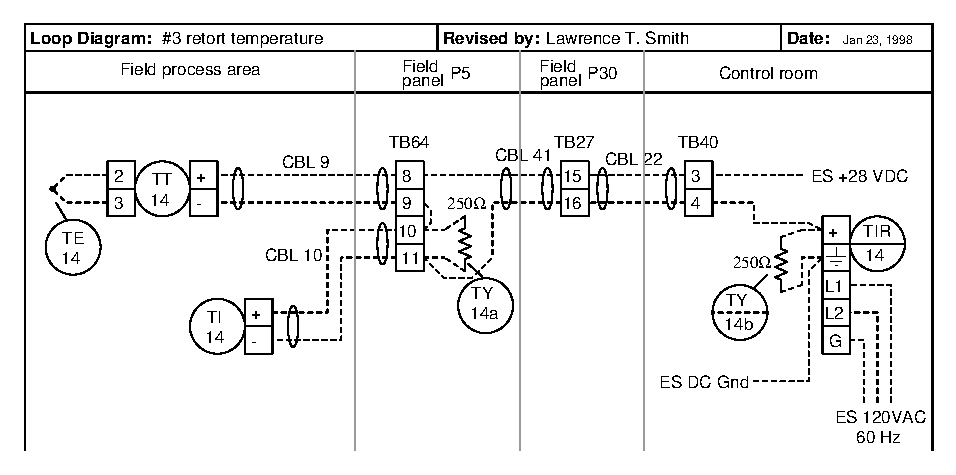
\includegraphics[width=15.5cm]{i00378x05.eps}$$


%INDEX% Lab exercise, temperature measurement loop

%(END_NOTES)
